\chapter{Konzeption}
\label{ch:Konzeption3}

Dieses Kapitel beschreibt die Konzeptionsphase des Prototypen, mit dem der Ansatz dieser Thesis geprüft wird. Hierzu werden in Kapitel \ref{sec:Anwendungsfalle3} Anwendungsfälle  definiert, um anschließend in Kapitel \ref{sec:usecase1} und \ref{sec:usecase2} relevante Themenfelder, zur Implementierung des Prototypen, auf Basis der Anwendungsfälle zu identifizieren. Die identifizierten Themenfelder bilden das technische Konzept zur Implementierung des Prototypen, der in Kapitel \ref{ch:implementierung4} dargestellt wird.

\section{Definition von Anwendungsfällen}
\label{sec:Anwendungsfalle3}

Dieser Abschnitt erläutert die Wahl der Anwendungsfälle , die in dieser Arbeit für die Konzeption und Implementierung verwendet werden. Die beiden auserwählten Anwendungsfälle \emph{Erkennung von Kreditausfällen} und \emph{Erkennung von Betrugsversuchen} werden in Kapitel \ref{subsec:Kreditausfallen3} bzw. \ref{subsec:Banktransaktionen3} im Detail erläutert. Darüber hinaus werden für jeden Anwendungsfall Szenarien definiert, mit denen das Potenzial von Online-Learning überprüft wird.   

Die Anwendungsfälle wurden anhand der nachfolgenden Kriterien ausgewählt:  

\begin{itemize*}
\item \textbf{Allgemeingültigkeit:} Der Anwendungsfall muss generischer Natur sein, so dass ein entwickeltes Verfahren zur Lösung des Anwendungsfalls in verschiedenen Unternehmen und Branchen angewendet werden kann.      
\item \textbf{Realitätsbezug:} Der Anwendungsfall muss in seiner Komplexität repräsentativ dafür stehen, was auch in realen Softwareentwicklungsprojekten an Komplexität abverlangt wird.     
\item \textbf{Stellenwert des Anwendungsfalls:} Ein möglicher Anwendungsfall muss einen gewissen Stellenwert innerhalb einer Branche besitzen, so dass neue, besser funktionierende Verfahren einen messbaren wirtschaftlichen Mehrwert schaffen.
\item \textbf{Automatisierte Entscheidungen:} Kern eines möglichen Anwendungsfalles muss das Treffen einer automatisierten operativen Entscheidung sein. Typischerweise gibt es bereits Lösungen, die auf Technologien, wie Business Process Management, Business Rules Management oder Decision Management, aufsetzen.  
\end{itemize*}

Anhand dieser Kriterien wurden die beiden Anwendungsfälle Erkennung von Kreditausfällen, sowie Erkennung von Betrugsversuchen bei Kreditkartentransaktionen, als am besten geeignet identifiziert. Darüber hinaus wurden auch die Anwendungsfälle Erkennung von Geldwäsche, sowie die Erkennung von Marktmanipulationen evaluiert und als weniger geeignet eingestuft, da beide Anwendungsfälle eher regulatorischen Zwecken dienen und weniger dem Kerngeschäft der Banken.   

\subsection{Erkennung von Kreditausfällen}
\label{subsec:Kreditausfallen3}

Wie in Kapitel \ref{ch:Motivation1} bereits beschrieben, können Kredite, die nicht zurückgezahlt werden, zu hohen Verlusten bei Banken führen. Dies wiederum kann zu Finanzkrisen führen, die die komplette Weltbevölkerung in ihren Auswirkungen erreicht. Daher ist die korrekte Erkennung des Kreditrisikos ein elementarer Bestandteil des Kreditvergabeprozesses und maßgeblich verantwortlich für dessen Qualität. Die Eigenkapitalvorschrift Basel II ist für alle Banken in Mitgliedsländern der Europäischen Union verpflichtend \cite{RE13} und hält darüber hinaus fest, wie Kreditrisiken zu berechnen sind. Abbildung \ref{fig:creditriskdimensions} \cite{GK10} zeigt die Hauptkomponenten zur Berechnung des Kreditrisikos. 

\begin{figure}[ht]
\centering
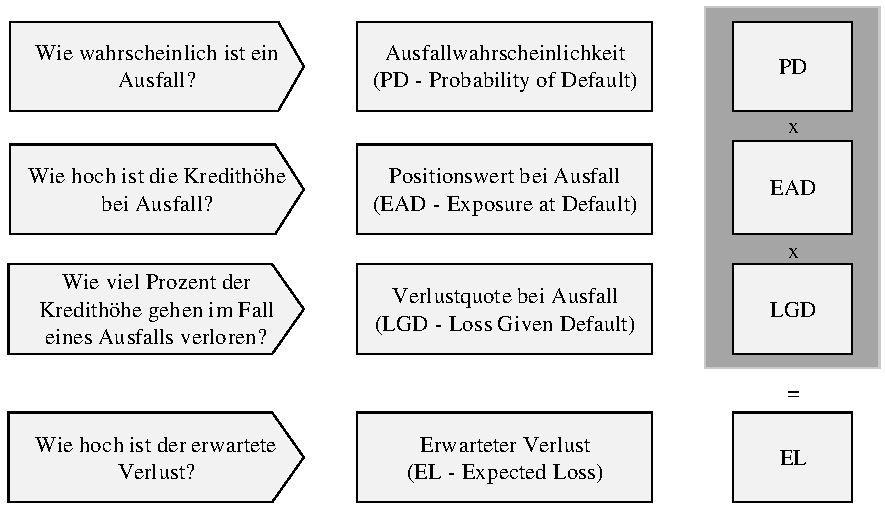
\includegraphics{images/creditriskdimensions.pdf}
\caption{Die Hauptkomponenten des Kreditrisikos.}
\label{fig:creditriskdimensions}
\end{figure}   

Der erwartete Verlust (EL) bildet die Grundlage zur Bestimmung der Eigenkapitalanforderung an die Bank nach Basel II \cite[vgl. S. 31]{ER11}. Dabei hat das Kreditinstitut die Freiheit Modele zur Errechnung der Ausfallwahrscheinlichkeit (PD) selbst zu bestimmen, so lange spezifische Minimalanforderungen erfüllt werden. Basel II nennt keine bevorzugte Methode, oder Best-Practice zur Erstellung eines Models. Engelmann und Rauhmeier \cite{ER11} nennen die Regressions- und Diskriminanzanalyse als die gängigsten Verfahren zur Modelbildung im Umfeld der Kreditvergabe. 

Neben der Berechnung quantitativer Faktoren, fließen auch qualitative Faktoren in die Kreditentscheidung mit ein \cite[vgl. S. 25 ff.]{NB04}. Insbesondere bei Krediten an Firmenkunden besitzt die Betrachtung der qualitativen Faktoren einen, hohen Stellenwert. Als Beispiel für mögliche qualitative Faktoren wäre die Branche des Unternehmens oder die Erfahrung des Managements zu nennen. Im klassischen Privatkunden-Kreditgeschäft sind komplett automatisierte Bewertungsverfahren die Regel \cite[vgl. S. 31 ff.]{NB04}. Unabhängig vom  Kreditvergabeprozess als Ganzes muss bei Firmenkunden, wie Privatkunden, die Ausfallwahrscheinlichkeit ermittelt werden. 

Um das Potenzial von Online-Learning (vgl. Kapitel \ref{sec:Machine_Learning2}) aufzuzeigen, werden für diesen Anwendungsfall die nachfolgende Szenarien definiert:   

\begin{itemize*}
\item \emph{Ausfall von Krediten mit schlechtem Einkommen-Schulden-Verhältnis.} Das Einkommen-Schulden-Verhältnis ist eine aussagekräftige Bemessung der Bonität. Das Szenario sieht vor, dass die Kunden mit dem schlechtesten Einkommen-Schulden-Verhältnis, ihre Kredite nicht mehr stemmen können. Hierbei gibt es eine große Parallele zur Finanzkrise, den dadurch dass die Häuser zu wertvoll bewertet wurden, stimmte die errechnete Bonität des Kunden nicht mehr und Kredite fingen an auszufallen. Ähnlich wie bei der Finanzkrise, wird im hier gewählten Szenario ein Fehler in den Eingabe-Daten simuliert.
\item \emph{Ausfall von Krediten die an Mieteinnahmen gebunden sind.} Das zweite Szenario sieht vor, dass Kredite, die an Wohnungen mit mehreren Wohneinheiten gekoppelt sind, vermehrt ausfallen. Dabei wird unterstellt, dass manche Häuser mittels Mieteinnahmen finanziert werden. Durch den Ausfall der Mieteinnahmen kommt es zu einem Liquiditätsverlust des Kreditnehmers, was im Ausfall des Kredites endet. Dieses Szenario simuliert den Eintritt zufälliger Ereignisse aus der Wirtschaft, die großen Einfluss auf die zu treffende Entscheidung haben. 
\end{itemize*}

\subsection{Erkennung von Betrugsversuchen}
\label{subsec:Banktransaktionen3}

Der zweite Anwendungsfall ist das Erkennen von betrügerischen Banktransaktionen. Studien wie \cite{FB11} zeigen, dass durch Kreditkartenbetrug in den Vereinigten Staaten im Jahr 2009, ein Schaden von 190 Milliarden Dollar entstanden ist. Ebenso zeigen Studien \cite[vgl. S. 24]{LE16}, dass im Jahr 2016 66 \% aller Betrugsversuche erfolgreich sind. 

ACTICO bietet in ihrer Compliance-Lösung \cite{AC17} das Modul Name Matching Transaction (NMT) \cite{AN17} an. Das NMT Modul prüft vor der Ausführung einer Banktransaktion, ob ein Betrugsverdacht vorliegt. Sollte eine Transaktion als verdächtig eingestuft werden, wird die Ausführung vorübergehend angehalten. In diesem Zeitraum nimmt die Bank Kontakt mit dem Kunden auf und prüft, ob die Transaktion so von ihm gewollt war und wieder freigegeben werden darf. 

Eine Transaktion verbindet zwei Parteien, den Auftraggeber der Transaktion und den Empfänger der Transaktion. Sind beide Parteien Kunde der selben Bankinstitution ist keine Prüfung notwendig, da die Transaktion, im Falle eines Betrugs, problemlos widerrufen werden könnte. Sind die beiden Parteien Kunden verschiedener Bankinstitutionen (Entscheidung "`Check fraud relevance"' in Abbildung \ref{fig:fraud-dmn}) beginnt die eigentlich Betrugsprüfung.  

\begin{figure}[ht]
\centering
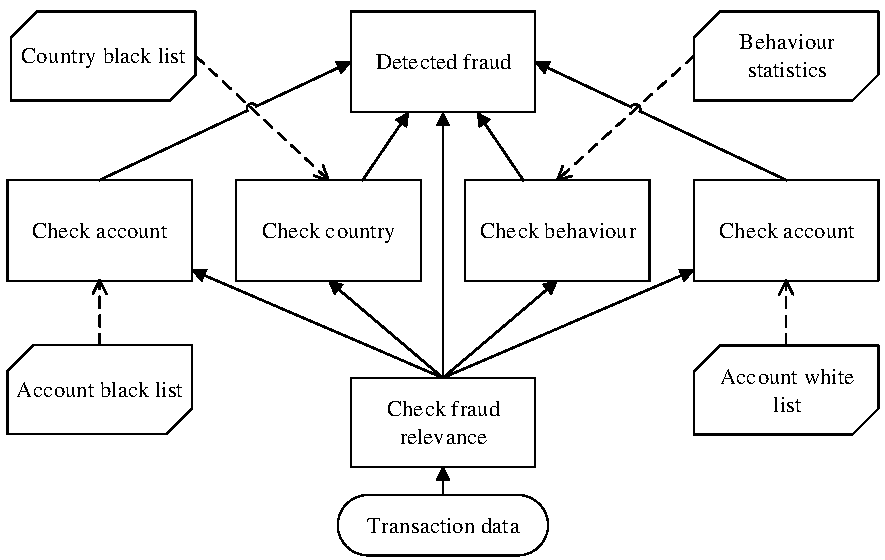
\includegraphics{images/fraud-dmn.pdf}
\caption{Decision Requirements Diagram der Transaktionsbetrugs-Entscheidung.}
\label{fig:fraud-dmn}
\end{figure}

Die anschließend ausgelöste Betrugsprüfung besteht aus vier Entscheidungen:

\begin{itemize*}
\item \textbf{Check account (Black-List):} Ein Betrugsfall liegt vor, wenn der Empfänger auf einer "`Black-List"' steht. Derartige Prüflisten werden von öffentlichen Ämtern aber auch von kommerziellen Anbietern veröffentlicht. 
\item \textbf{Check country:} Ein Betrugsfall liegt vor, wenn das Ziel-Land des Empfängers auf einer Prüfliste steht. 
\item \textbf{Check behaviour:} Ein Betrugsfall liegt vor, wenn Abweichung in den Nutzungs-Statistiken des Kunden entdeckt wurden. Hierzu zählen ungewöhnliche Zahlungsmethoden, Abweichungen von den üblichen Transaktionszeiten, Abweichungen zu den üblichen Beträgen vorheriger Transaktionen und Abweichungen von der üblichen Menge an Transaktionen in einem Monat.
\item \textbf{Check account (White-List):} Ein Betrugsfall liegt nicht vor, wenn der Empfänger auf einer "`White-List"' steht. Eine White-List ist eine Liste mit Bankkonten die als vertrauenswürdig eingestuft wurden. Transaktionen die der Bank-Kunde nachträglich freigeben hat, werden anschließend der White-List hinzugefügt. 
\end{itemize*}

Die letzte Entscheidung "`Fraud detected"' empfängt die Ergebnisse der vorangegangenen Entscheidungen. Sollte bei keiner der vorangegangenen Entscheidung einen Verdacht auf Betrug vorliegen, liegt kein Betrug vor, selbst wenn der Transaktions-Empfänger nicht auf der White-List steht. Sollte nur eine der Entscheidungen einen Betrugsverdacht an "`Fraud detected"' leiten, wird die komplette Transaktion gesperrt. Üblicherweise folgt bei Kunden von ACTICO an dieser Stelle einen Workflow, der den Bankkunden per SMS über die Sperrung informiert. Der Bankkunde kann die Transaktion anschließend auf seinem Mobiltelefon wieder freigeben (Transaktionen in Embargo-Länder, oder von Sanktionen betroffene Länder, können nicht wieder freigegeben werden).    

\section{Model zur Erkennung von Kreditausfällen}
\label{sec:usecase1}

Im nachfolgenden Kapitel werden alle relevanten Themenfelder zur prototypischen Realisierung des ersten Anwendungsfalls vorgestellt. Zur Bildung eines Models, dass ausfallende Kredite identifizieren kann, müssen zuerst Lerndaten generiert werden  (Kapitel \ref{subsec:Lerndaten31}). Die Lerndaten ermöglichen anschließend das Lernen unter Verwendung eines ML-Algorithmus, der mittels des Lernprozesses das Model bildet (Kapitel \ref{subsec:Neuro31}).

\subsection{Lerndaten}
\label{subsec:Lerndaten31}

Nach ausgiebiger Recherche konnten, über ein Webportal des amerikanischen Hypotheken-Rückversicherer Fannie Mae, geeignete anonymisierte Kreditantragsdaten gefunden werden \cite{FM17}. Alle Datensätze entstammen Immobilien-Darlehen. Die Kreditantragsdatensätze sind über Identifikationsnummern mit Performancedatensätzen verbunden, die das Zahlungsverhalten und weitere Informationen monatlich erfassen \cite{FM18}. 

\paragraph{Datenerzeugung.} Zum Download stehen die Acquisition- (Kreditantragsdaten) und die Performance-Datei (Performancedaten) bereit. Der erste Schritt zur Modellbildung ist die Aufbereitung der Lerndaten. Diese bestehen aus Features und einem Label (vgl. Kapitel \ref{sec:Machine_Learning2}). Als Features dienen die Kreditantragsdaten aus der Acquisition-Datei, durch den Prozess des Feature Engineerings (siehe Exkurs \ref{def:engineering}) aufbereitet werden. Um die Erzeugung der Lerndaten abzuschließen muss noch das Label ermittelt werden. Das Label, beschreibt die Erfahrung aus der Vergangenheit, aus der gelernt werden soll. Im vorliegenden Anwendungsfall bedeutet dies konkret, ob der Kredit ausgefallen ist oder nicht. Zur Ermittlung des Labels eines Kreditantragsdatensatz muss die Performance-Datei auf Zahlungsverzögerungen untersucht werden. 

\begin{definition}[\textbf{Feature Engineering}]
\begin{shaded}
\emph{''Feature Engineering} is the process of transforming raw data into features that better represent the underlying problem to the predictive models, resulting in improved model accuracy on unseen data.'' \cite{MM17}. Feature Scaling und Feature Selection sind Teilmengen des Feature Engineerings. Zusammenfassend lässt sich festhalten, dass der Prozess der Transformation von Attributen aus den Rohdaten, zu Features die dem ML-Algorithmus verständlich sind, als Feature Engineering bezeichnet wird. 
\label{def:engineering}
\end{shaded}
\end{definition}

Jeder Kreditantragsdatensatz besitzt eine einzigartige Identifikationsnummer. Mittels dieser Identifikationsnummer können alle Performancedatensätze zu jenem Kredit identifiziert werden. Die Performancedatensätze sind mit Zeitstempeln gekennzeichnet, wobei der aktuellste Datensatz verwendet wird um den Zahlungsverzug, und damit das gesuchte Label, festzustellen. Die Spalte \textit{Current Loan Delinquency Status} beziffert den aktuellen Zahlungsverzug in Monaten. Befindet sich der Kunde in Zahlungsverzug (Current Loan Delinquency Status > 0) wird dem Label der Wert 1 zugewiesen (Ausfall des Kredites). Liegt kein Zahlungsverzug vor (Current Loan Delinquency Status = 0), wird der Wert 0 zu gewiesen (kein Ausfall des Kredites). Wenn der Zahlungsverzug unbekannt ist, besitzt Current Loan Delinquency Status den Wert ''X''. In diesem Fall werden die betroffenen Datensätze übersprungen. Abbildung \ref{fig:cleansing} soll den Prozess der Lerndatenerzeugung nochmals veranschaulichen.

\begin{figure}[ht]
\centering
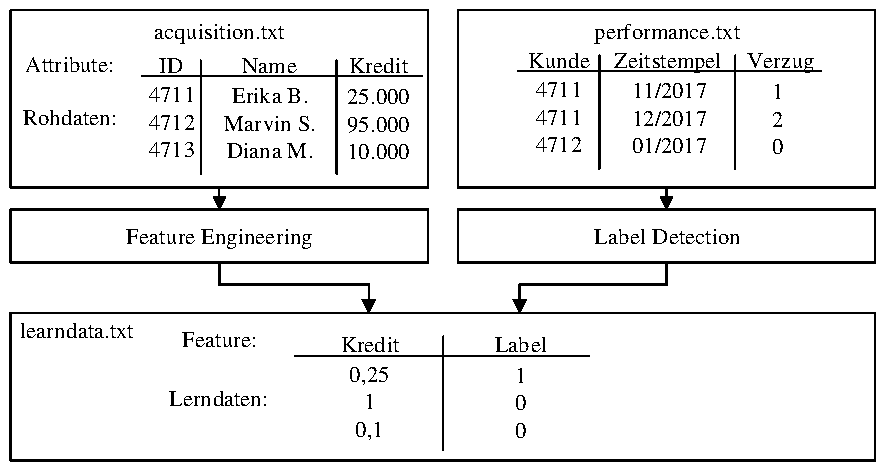
\includegraphics{images/cleansing.pdf}
\caption{Vorgehensweise bei der Erstellung des Lerndatensatzes.}
\label{fig:cleansing}
\end{figure}  

Zusammenfassend sollte festgehalten werden, dass zur Bildung des Lerndatensatzes zwei Prozesse ablaufen müssen. Einer zur Bildung der Features, durch die Durchführung von Feature Engineering. Der andere Prozess, generiert das Label aus der Performancedatei (Nach dem oben beschriebenen Verfahren). 
 
Im vorliegenden Anwendungsfall wurde Feature Engineering genutzt, um kategorische Attribute in ein Format zu überführen, so dass das neuronale Netz das Feature als kategorischen Wert und nicht als nummerischen Wert interpretiert. Hierzu muss jede mögliche Klasse eines Attributes auf ein eigenes Feature abgebildet werden. Beispielsweise bedeutet das, dass aus dem Attribut Bundesstaat in den Ausgangsdaten, für jeden möglichen Wert ein Feature extrahiert werden muss. Die Vereinigten Staaten von Amerika besitzen 50 Bundesstaaten, dementsprechend wird das Attribut Bundesstaat in den Ausgangsdaten auf 50 Features in den Lerndaten zerlegt. Der Inhalt des Features, bildet ein boolescher Wert, der spezifiziert, ob der Kreditnehmer in diesem Bundesstaat lebt oder nicht. Nicht selten kommt es vor, dass ein Attribut in den Ausgangsdaten keinen Wert besitzt, also leer ist. Um dem neuronalen Netz diesen Sachverhalt verständlich zu machen wird ein weiteres Feature hinzugefügt, das einen booleschen Wert besitzt, der spezifiziert, ob der Bundesstaat im Kreditantragsdatensatz enthalten ist oder nicht. Tabelle  \ref{tab:feature-engine} illustriert das eben genannte Beispiel nochmals.   

\begin{table}[ht]
\centering
\small
\begin{tabular}{cccc}
\toprule
\ state-is-unknown & is-in-alabama & is-in-alaska & is-in-arizona\\\toprule
0 & 0 & 0 & 1\\\midrule
1 & 0 & 0 & 0\\\midrule
... & ... & ... & ...\\\bottomrule
\end{tabular}
\caption{Zerlegung des kategorischen Bundesstaat-Attributs in Features.}
\label{tab:feature-engine}
\end{table}

Die eben genannte Vorgehensweise wird auch auf alle anderen kategorischen Attribute angewandt. Je nach Datenbankschema, müssen für Werte die \glqq nullable\grqq{} sein dürfen, extra Features eingeführt werden, die dies entsprechend abbilden. Im vorliegenden Datensatz der Fannie Mae wurden die Attribute \emph{Channel}, \emph{First-Time-Home-Buyer-Indicator}, \emph{Loan Purpose}, \emph{Property Type}, \emph{Occupancy Status}, \emph{Property state} und \emph{Co Borrower Credit Score} (vorhanden bzw. nicht vorhanden) kategorisch zerlegt. Somit ergeben sich aus den 18 Attributen der Rohdaten, 83 Features in den Lerndaten. Außerdem wurden die Attribute \emph{Origination Date} und \emph{First Payment Date} von einander subtrahiert. Ein Machine Learning Algorithmus, kann Daten im Datumsformat nicht zweckgemäß interpretieren. Aus diesem Grund wurde die Differenz in Monaten zwischen beiden Daten ermittelt und anschließend als Feature den Lerndaten hinzugefügt.   

\begin{definition}[\textbf{Feature Selection}]
\begin{shaded}
\emph{Feature Selection} beschreibt die Auswahl der aussagekräftigsten Features aus einem Datensatz \cite[vgl. S. 503 ff.]{SG17}. Aussagekräftig bedeutet in diesem Kontext, wie stark wirkt sich die Existenz des Features auf das zu berechnende Label aus. Der Kreditantragsdatensatz besteht aus vielen nützlichen Informationen zur Vorhersage der Ausfallwahrscheinlichkeit. Allerdings beinhalten solche Datensätze auch sekundäre Informationen, wie z.B. den Namen des Kreditnehmers. Aus dem Namen des Kreditnehmers kann kein Rückschluss auf dessen Ausfallwahrscheinlichkeit gezogen werden.   Daher macht es keinen Sinn, derartige Features mit in den Lerndatensatz aufzunehmen, da der Lerndatensatz und damit auch das neuronale Netz mehr Speicher und Rechenzeit benötigen würde. Zur Identifizierung der wichtigen Features gibt es grundsätzlich zwei Herangehensweisen: Die erste Herangehensweise identifiziert Features aufgrund von Domänenwissen im vorliegenden Anwendungsfall. Die zweite Herangehensweise ist die Durchführung einer Dimensionalitätsreduktion \cite[vgl. S. 326]{SG17}. Data Mining Tools wie Weka \cite{WEKA17} oder KNIME \cite{KNIME17} bieten Funktionen, die angeben, wie hoch der Einfluss eines Features auf das Label ist. 
\label{def:selection}
\end{shaded}
\end{definition}

Für den vorliegenden Datensatz wurden keine Dimensionalitätsreduktion durchgeführt, da die Acquisition-Datei, die die Kreditantragsdatensätze enthält, die geringe Anzahl von 25 Attributen aufweist. Eine Feature-Selection, aufgrund von Performance-Gründen, ist somit nicht notwendig. Allerdings wurden aufgrund von Domänenwissen die Attribute \emph{Mortage Insurance Percentage}, \emph{Product Type}, \emph{Mortage Insurance Type} und \emph{Relocation Mortage Indicator} ausgeschlossen. Diese Attribute enthalten ausschließlich Informationen über die von Fannie Mae bereitgestellte Rückversicherung und tragen somit nicht zur Erkennung eines Kreditausfalles bei. Darüber hinaus würde das Kriterium der Allgemeingültigkeit verletzt werden, sowie zur Fälschung der Ergebnisse beitragen, da Banken zum Zeitpunkt der Kreditvergabe nicht über derartige Informationen verfügen.    

\begin{definition}[\textbf{Feature Scaling}]
\begin{shaded}
\emph{Feature Scaling} beschreibt ein Verfahren bei dem Daten auf einen festgelegten Bereich skaliert werden \cite[vgl. S. 322]{SG17}. Typischerweise weichen die Daten in ihren Werten pro Spalte stark ab. Allerdings sollten alle Werte einer Spalte auf einen Bereich zwischen null und eins skaliert werden. Der Grund für die Notwendigkeit von Feature Scaling ist, dass das Gradientenverfahren, welches Teil der komplexen Hintergrundberechnungen neuronaler Netze und vieler anderer ML-Algorithmen ist, lokale Minima schneller findet, wenn sich die Input-Variablen im selben Bereich befinden \cite[vgl. S. 203]{CG15}. 
\label{def:scaling}
\end{shaded}
\end{definition}

Um das Gradientenverfahren beschleunigen zu können müssen die Kreditantragsdatensätze pro Feature (spaltenweise) skaliert werden. Die Skalierung der Daten geschieht unter Verwendung der Formel \ref{formula:rescaling}.  

\begin{align}
\label{formula:rescaling}
x' = \frac{x-min(x)}{max(x)-min(x)}
\end{align}

Die Skalierung wird immer pro Datenspalte vorgenommen, dazu wird zuerst der Größte wie der Kleinste Wert der Spalte berechnet, woraufhin anschließend die Formel auf jeden Wert der Spalte angewendet und durch $x'$ ersetzt wird.
Sicherheitshalber muss geprüft werden, dass $max(x)$ und $min(x)$ nicht gleich groß sind. Dies könnte dazu führen, dass versucht wird durch null zu teilen, was die Applikation zum Absturz bringen würde. Sollte $max(x)$ und $min(x)$ gleich groß sein, würde das bedeuten dass das Feature nur aus einem Wert besteht. Ein solches Feature wäre allerdings sinnlos, da es kein Rückschluss auf die zu identifizierende Klasse erlaubt. Ein solcher Fall sollte somit nie in der Realität auftreten. Nichts desto trotz muss der Prototyp eine entsprechende Fehlerbehandlung besitzen.

Die Kreditantragsdaten werden von Fannie Mae Quartalsweise veröffentlicht. Aus diesem Grund werden die Antragsdaten von Quartal eins bis drei, aus dem Jahr 2007 verwendet, um das Modell zu erlernen (Lerndaten). Die Akkuranz des erlernten Modells wird mittels der Daten aus Quartal vier überprüft (Evaluationsdaten). Es soll also untersucht werden, welche Vorhersagen für Quartal vier getroffen werden. Die Vorhersagen werden anschließend verglichen mit den in echt eingetretenen Kreditausfällen.

Die in Kapitel \ref{subsec:Kreditausfallen3} vorgestellten Szenarien, werden durch die Manipulation der Lerndaten abgebildet. Für Szenario 1, wird anhand des Attributs \emph{Debt-to-inocme-ratio} in den Ausgangsdaten identifiziert, welche Kredite Ausfallen werden. Dazu wird das Label der Kredite, deren Debt-to-inocme-ratio den Wert fünfzig übersteigt, auf eins gesetzt (Ausgefallen). Für Szenario 2, wird anhand des Attributs \emph{Number of Units} geprüft, welche Kredite ausfallen werden. Alle Kredite, deren Number of Units größer vier ist, werden in Szenario 2 ausfallen. 

\subsection{Modellbildung}
\label{subsec:Neuro31}

Nach der Erzeugung der Lerndaten, kann ein Algorithmus konzipiert werden, der aus den Lerndaten ein Modell zur Vorhersage von Kreditausfällen erlernt. Hierzu soll ein mehrschichtiges neuronales Netz verwendet werden. Aus den Lerndaten, ergibt sich die Anzahl an Eingabe- und Ausgabe-Neuronen. Die Lerndaten besitzen 83 Features, somit besteht die Eingabe-Schicht aus 83 Neuronen. Aufgrund der Anzahl möglicher Werte für das Label, Kreditausfall oder kein Kreditausfall, ergibt sich die Anzahl zwei für die Ausgabe-Neuronen. Somit steht die Architektur der Ein- und Ausgabeschicht fest und es gilt die Anzahl der versteckten Schichten, sowie die Anzahl der Neuronen innerhalb der versteckten Schichten, zu bestimmen. Die Wahl dieser Parameter ist komplex und wirkt sich immens auf das Lernverhalten des neuronalen Netzes aus. 

\begin{definition}[\textbf{Underfitting vs. Overfitting}]
\begin{shaded}
\emph{Underfitting} beschreibt den Sachverhalt, dass ein Modell weder eine gute Performance bei den Lerndaten, noch bei neuen Datensätzen, aufweisen kann \cite{MM16}. Underfitting kann sehr leicht erkannt werden. Entweder anhand des ausbleibenden Lernfortschritt während des Lernens, oder anhand schlechter Vorhersagen des Modells.   
\emph{Overfitting} \cite[vgl. S.947 ff.]{SG17} beschreibt den Sachverhalt, dass ein Modell die Lerndaten so exakt widerspiegelt, dass das Modell neue, unbekannte Datensätze nicht mehr korrekt vorhersagen kann. Das bedeutet, dass das Modell eine sehr geringe Fehlerrate gegenüber den Lerndaten, mit denen das Modell erlernt wurde, aufweist. Neue Datensätze allerdings, resultieren in sehr hohen Fehlerraten. Als Entwickler gilt es also ein Modell zu entwickeln, das sich in einem Optimum zwischen beiden Extremen befindet. 
\label{def:fitting}
\end{shaded}
\end{definition}

Bei der Wahl der Architektur, müssen die Parameter (Anzahl versteckte Schichten und Anzahl Neuronen pro versteckte Schicht) so gewählt werden, dass Under- wie auch Overfitting verhindert wird. Bezüglich des Vorgehens zur Wahl dieser Netzwerkparameter, ist sich die Wissenschaft uneinig. Publikationen wie \cite{Blum92, Swingler96, Berry97} stellen Daumenregeln zur Wahl der Netzwerkparameter bereit. Blum behauptet \cite{Blum92} die Anzahl der Neuronen in den versteckten Schichten, sollte zwischen der Anzahl an Eingabe- und Ausgabe-Neuronen liegen. Swingler \cite{Swingler96}, wie auch Berry und Linoff \cite{Berry97} beteuern, dass sich niemals mehr Neuronen in einer versteckten Schicht befinden sollten, als die doppelte Anzahl der Eingabe-Neuronen. Andere Quellen \cite{FAQ14} bezeichnen diese Daumenregeln als nutzlos, da andere wichtige Faktoren, wie beispielsweise die Anzahl der Lerndatensätze, außer Acht gelassen werden. Elisseeff und Paugam-Moisy stellen in ihrer Publikation "`Size of multilayer networks for exact learning: analytic approach"' \cite{EPM97} ein Theorem, zur Berechnung der unteren und oberen Grenze der Anzahl Neuronen vor. Im Gegensatz zu den Ansätzen von \cite{Blum92, Swingler96, Berry97}, werden im Ansatz von Elisseeff und Paugam-Moisy, auch die Anzahl an Lerndatensätzen betrachtet. Darüber hinaus, treffen Elisseeff und Paugam-Moisy keine Aussage über die optimale Anzahl versteckter Neuronen, sondern bieten eine Formel zur Berechnung der minimal notwendigen (Formel \ref{formula:lowbound}), beziehungsweise maximal ausreichenden Anzahl an Neuronen (Formel \ref{formula:upbound}). 

\begin{align}
\label{formula:lowbound}
 N_{H} = \left[\frac{N_{P}N_{S}}{N_{I}+N_{S}} \right] 
\end{align}

\begin{align}
\label{formula:upbound}
 N_{H} = 2\left[\frac{N_{P}N_{S}}{N_{I}+N_{S}} \right]N_{S}
\end{align}   

Dabei beschreibt $N_{P}$ die Anzahl der Lerndatensätze, $N_{S}$ die Anzahl der Ausgabeneuronen (bzw. die Anzahl möglicher Labels) und $N_{I}$ die Anzahl der Eingabeneuronen (bzw. die Anzahl der Features des Lerndatensatzes). Für diesen Lerndatensatz, ergibt sich unter der Verwendung von $N_{P} = 100000$, $N_{S} = 2$ und $N_{I} = 83$ einen Wert von $N_{H}\approx2350$ notwendigen Neuronen pro Schicht (nach Formel \ref{formula:lowbound}).  

Nun gilt es die Anzahl der versteckten Schichten zu bestimmen. Zur Abbildung eines linearen Problems, ist eine Ein- und Ausgabe-Schicht schon ausreichend \cite{MN89}. Zur Erlernung komplexer, nicht linearen Zusammenhängen müssen, abhängig von den gewählten Aktivierungsfunktionen, mindestens ein bis zwei versteckte Schichten verwendet werden \cite{FAQ15, LA09}.   

\begin{definition}[\textbf{Vanishing Gradient Problem}]
\begin{shaded}
\emph{Vanishing Gradient Problem} beschreibt ein Problem, das beim Lernen, unter der Verwendung mehrschichtiger neuronale Netze, auftritt. Das Problem besteht darin, dass bei der Verwendung von $n$-Schichten die Fehlerrate,  mittels der die Gewicht-Updates berechnet werden, exponentiell mit $n$ sinkt. Dies führt zu einem langsameren Lernverhalten in den vorderen Schichten und dadurch, zu einem generell schlechteren, oder sogar ausbleibendem Lernverhalten. Sepp Hochreiter \cite{SH91} beschrieb das Vanishing Gradient Problem 1991 als Erster. Es gilt bis heute, als große Herausforderung bei der Verwendung (mehrschichtiger) neuronaler Netze.        
\label{def:vanishing}
\end{shaded}
\end{definition}

Um dem Vanishing Gradient Problem entgegen zu wirken, werden in diesem Anwendungsfall, so wie in \cite{FAQ15, LA09} empfohlen, zwei versteckte Schichten verwendet. Sollte festgestellt werden, dass zwei Schichten nicht ausreichend sind um die Komplexität des abzubildenden Problems festzuhalten, könnte gegebenenfalls ein Benchmark mit einem dreischichtigen neuronalen Netz durchgeführt werden. 

\begin{definition}[\textbf{Regularisierung}]
\begin{shaded}
\emph{Regularisierung} beschreibt Techniken, deren Ziel es ist Overfitting (siehe Exkurs \ref{def:fitting}) zu verhindern \cite{QU17}.
\label{def:regularization}
\end{shaded}
\end{definition} 

Dahl et al. \cite{DA13} empfehlen die Kombination der Regularisierungs-Techniken \emph{Early stopping} und \emph{Dropout} zur Verhinderung von Overfitting. Beide Techniken könnten auch einzeln verwendet werden, allerdings beweisen Dahl et al., dass sich durch die Kombination der Techniken die Fehlerrate der Vorhersagen des Modelles zusätzlich verbessert.

\begin{definition}[\textbf{Early stopping}]
\begin{shaded}
\emph{Early stopping} beschreibt eine Technik, zur Verhinderung von Overfitting. Typischerweise wird vor dem Lernen des Netzes spezifiziert, wie oft der komplette Lerndatensatz das neuronale Netz passiert (Epoche). Wird der Parameter zu klein gewählt, könnte Underfitting eintreten. Wird er zu groß gewählt, könnte Overfitting eintreten. Early Stopping übernimmt die manuelle Wahl der Anzahl an Epochen, indem ein Teil der Lerndaten in einen Testdatensatz überführt wird. Anschließend werden nach jeder Epoche, die Vorhersagen des Models auf den Testdatensatz geprüft. Haben sich die Vorhersagen des Models in dieser Epoche verbessert, überschreibt der Algorithmus das alte Model und beginnt eine neue Epoche. Wenn nicht behält er das alte Model, verwirft das neu erlernte Model und beginnt eine neue Epoche.  
\label{def:early}
\end{shaded}
\end{definition} 

Die bereits generierten Lerndaten, wurden für die Umsetzung von Early Stopping aufgeteilt. Hierzu werden die Datensätze der Lerndaten zuerst gemischt, so dass diese nicht mehr in einer zeitlichen Reihenfolge stehen. Anschließend werden 10000 Datensätze aus den Lerndaten ausgeschnitten und in eine weitere Textdatei kopiert, diese Datensätze werden ausschließlich zur Regularisierung mittels Early stopping verwendet. 

Die nächsten Abschnitte:

Dropout

Zusammenfassung plus Überleitung

\section{Modell zur Erkennung von Betrugsversuchen}
\label{sec:usecase2}

\subsection{Lerndaten}
\label{subsec:Lerndaten32}


\subsection{Modellbildung}
\label{subsec:Neuro32}